\input{/Users/daniel/github/config/preamble-por.sty}%available at github.com/danimalabares/config
%\input{/Users/daniel/github/config/thms-por.sty}%available at github.com/danimalabares/config

\newcommand{\rightlooparrow}{\mathbin{
    \vbox{\openup-10.25pt\halign{\hss$##$\hss\cr\circ\cr\longrightarrow\cr}}
}}

\begin{document}
\bibliographystyle{alpha}
\begin{minipage}{\textwidth}
	\begin{minipage}{1\textwidth}
		\hfill Daniel González Casanova Azuela
		
		{\small Prof. Luis Florit\hfill\href{https://github.com/danimalabares/rg}{github.com/danimalabares/rg}}
	\end{minipage}
\end{minipage}\vspace{.2cm}\hrule

\vspace{10pt}
{\huge Exercícios de Geometria Riemanniana}
\tableofcontents

\section{Exercícios do do Carmo}

\subsection{Capítulo 0}
\begin{thing4}{Exercise 2}\label{exer:2}\leavevmode
Prove que o fibrado tangente de uma variedade diferenciável \(M\) é orientável (mesmo que \(M\) não seja).
\end{thing4}

\begin{proof}[Solution]\leavevmode
Es porque la diferencial de los cambios de coordenadas está dada por la identidad y una matriz lineal. Sí, porque por definición las trivializaciones locales de \(TM\) preservan la primera coordenada \textbf{y} son isomorfismos lineales en la parte del espacio vectorial. Entonces queda que 
\[d(\varphi_U \circ \varphi_V^{-1})=\left(\begin{array}{@{}c|c@{}}
\operatorname{Id}&0\\
\hline
0&\xi \in \mathsf{GL}(n)\end{array}\right)\]
pero no estoy seguro de por qué \(\xi\) preservaría orientación, i.e. que tenga determinante positivo… a menos de que… 
\end{proof}

\begin{thing4}{Exercise 5}[Mergulho de \(P^2(\mathbb{R})\) em \(\mathbb{R}^4\) ]\label{exer:5}\leavevmode
Seja \(F:\mathbb{R}^3 \to \mathbb{R}^4\) dada por
\[F(x,y,z)=(x^2-y^2,xy,xz,yz),\qquad (x,y,z) = p \in \mathbb{R}^3.\]
Seja \(S^2 \subset \mathbb{R}^3\) a esfera unitária com centro na origem \(0 \in \mathbb{R}^3\). Oberve que a restrição \( \varphi:= F|_{S^2}\) é tal que \(\varphi(p)=\varphi(-p)\), e considere a aplicação \(\tilde{\varphi}:\mathbb{R}P^2 \to \mathbb{R}^4\) dada por
\[\tilde{ \varphi}([p])=\varphi(p),\qquad [p]\text{=clase de equivalência de \(p=\{p,-p\}\)} \]

Prove que
\begin{enumerate}[label=(\alph*)]
\item \(\tilde{\varphi}\) é uma imersão.
\item \(\tilde{\varphi}\) é biunívoca; junto com (a) e a compacidade de  \(\mathbb{R}P^2\), isto implica que \(\tilde{ \varphi}\) é um mergulho.
\end{enumerate}
\end{thing4}

\begin{proof}[Solution]\leavevmode
\begin{enumerate}[label=(\alph*)]
\item Considere a carta \(\{z=1\}\). A representação coordenada de \(\tilde{\varphi}\) vira
	\[(x,y) \longmapsto (x^2-y^2,xy,x,y)\]
cuja derivada como mapa \(\mathbb{R}^2 \to \mathbb{R}^4\) é
\[\begin{pmatrix} 2x& -2y\\y&x\\1&0\\0&1 \end{pmatrix} \]
que é injetiva. Agora pegue a carta \(\{x=1\}\). Então a representão coordenada de \(\tilde{ \varphi}\) vira
\[(y,z) \longmapsto (1-y^2,y,z,yz)\]
e tem derivada
\[\begin{pmatrix} -2y&0\\1&0\\0&1\\z&y \end{pmatrix} \]
que também é injetiva. Seguramente algo análogo acontece na carta \(\{y=1\}\).

\item \(\tilde{\varphi}\) é injetiva. Pegue dois pontos \(p_1:=[x_1:y_1:z_1]\) e \(p_2:=[x_2:y_2:z_2]\) e suponha que \(\tilde{\varphi}(p_1)=\tilde{\varphi}(p_2)\). I.e.,
	\[x_1^2-y_1^2=x_2^2-y_2^2,\qquad x_1y_1=x_2y_2,\qquad x_1z_1=x_2z_2, \qquad y_1z_1=y_2z_2\]
	Suponha primeiro que \(z_1 \neq  0\). Segue que
	\[x_1=\frac{z_2}{z_1}x_2, \qquad y_1=\frac{z_2}{z_1}y_2\]
	logo
	\[x_2^2-y_2^2=x_1^2-y_1^2=\left(\frac{z_2}{z_1}\right)^2(x_2^2-y_2^2)\implies z_2=z_1\implies x_1=x_2,\qquad y_1=y_2\]
	

	Em fim, uma imersão injetiva com domínio compacto é um mergulho porque é fechada: pegue um fechado no domínio, vira compacto, imagem é compacta, que é fechado. Pronto.
.
\end{enumerate}
\end{proof}

\begin{thing4}{Exercício 8}\label{exer:8}\leavevmode
\(\varphi:M_1\to M_2\) difeo local. Se \(M_2\) é orientável, então \(M_1\) é orientável.
\end{thing4}
\begin{proof}[Solução]\leavevmode
Defina: uma base \(\beta \subset T_pM\) é orientada se \(\varphi_*\beta\) é orientada em \(T_{\varphi(p)}M\). Tá bem definida porque \(\varphi\) é um difeomorfismo em \(p\), i.e. \(\varphi_*\) é isomorfismo. Para mostrar que é contínua à la Lee, qualquer vizinhança de um ponto \(p \in M_1\), a correspondente carta coordenada em \(\varphi(p)\), um marco coordenado nela e puxe (pushforward baix \(\varphi^{-1}\)) de volta para \(U\). Difeomorfismo e muito bom: o pushforward the campos vetoriais está bem definido. E por construção está orientado.
\end{proof}
\subsection{Capítulo 1}

\begin{thing4}{Exercise 1}\label{exer:1}\leavevmode
Prove que a aplicação antípoda \(A:S^n \to S^n\) dada por \(A(p)=-p\) é uma isometria de \(S^n\). Use este fato para introduzir uma métrica Riemanniana no espaço projetivo real \(\mathbb{R}P^{n}\) tal que a projeção natural \(\pi: S^n \to \mathbb{R}P^{n}\) seja uma isometria local.
\end{thing4}
\begin{proof}[Solution]\leavevmode
	Lembre que a métrica de \(S^n\) é a induzida pela métrica euclidiana, onde pensamos que \(T_pS^n \hookrightarrow T_p\mathbb{R}^{n+1}\). É claro que \(A\) é uma isometría de \(\mathbb{R}^n\), pois ela é a sua derivada (pois ela é linear), de forma que \(\left<v,w\right>_p=\left<-v,-w\right>_{A(p)}=\left<v,w\right>_{-p}\).

	É um fato geral que se as transformações de coberta preservam a métrica, obtemos uma métrica no quociente de maneira natural, i.e. para dois vetores \(v,w\in T_p\mathbb{R}P^n\) definimos \(\left<v,w\right>_p^{\mathbb{R}P^n}:=\left<\tilde{v},\tilde{w}\right>_{\tilde{p} \in \pi^{-1}(p)}\).

Para ver que a projeção natural é uma isometria local basta ver que a diferencial de \(A\) é um isomorfismo em cada ponto. Mas como ela é \(-A\), isso é claro.
\end{proof}

\begin{thing4}{Exercício 7}\label{exer:7}\leavevmode
Seja \(G\) um grupo de Lie compacto e conexo (\(\dim(G)=n\)). O objetivo do exercício é provar que \(G\) possui uma métrica bi-invariante. Para isto, prove as seguintes etapas:
\begin{enumerate}[label=(\alph*)]
\item Seja \(\omega\) uma \(n\)-forma diferencial em \(G\) invariante à esquerda, isto é, \(L_x^*\omega=\omega\), para todo  \(x\in G\). Prove que \(\omega\) é invariante à direita.

	\textit{Sugestão}: Para cada \(a \in Ga\), \(R_a ^*\omega\) é invariante à esqueda. Decorre daí que \(R_a ^*\omega=f(a)\omega\). Verifique que \(f(ab)=f(a)f(b)\), isto é, \(f:G \to \mathbb{R}\setminus\{0\}\) é um homomorfismo (contínuo) de \(G\) no grupo multiplicativo dos números reais. Como \(f(G)\) é um subgrupo compacto compacto e conexo, conclui-se que \(f(G)=1\). Logo \(R_a ^*\omega=\omega\).
\item Mostre que existe uma \(n\)-forma diferencial invariante à esquerda \(\omega\) em \(G\).
\item Seja \(\left<\cdot,\cdot\right>\) uma métrica invariante à esquerda em \(G\). Seja \(\omega\) uma \(n\)-forma diferencial positiva invariante à esqueda em \(G\), é defina uma nova métrica Riemanniana \(\left<\left<\cdot,\cdot\right>\right>\) em \(G\) por
\begin{align*}\left<\left<u,v\right>\right>_p&=\int_G\left<(d R_x)_yu,(d R_x)_yv\right>_{yx}\omega,\\
	&x,y \in G,\qquad u,v \in T_yG
\end{align*}
Prove que \(\left<\left<\cdot,\cdot\right>\right>\) é bi-invariante.
\end{enumerate}
\end{thing4}
\begin{proof}[Solução]\leavevmode
\begin{enumerate}[label=(\alph*)]
\item 
\item 
\item Vou usar outra notação. Suponha que \(g\) é uma métrica invariante à esquerda em \(G\). Definimos
	\[\tilde{g}:=\int_{x \in G}(R_x^*g)\omega\]
	como operador \(\mathfrak{X}(G)\times \mathfrak{X}(G) \longrightarrow \mathcal{F}(G)\).

	\begin{thing8}{Lance final}\leavevmode
Essa definição tá errada! Para que \(R_x^*g\) seja uma função que acompanhe \(\omega\) em cada ponto, \textbf{também temos que puxar \(\omega\)}. Ou seja, a definição correta é:
	\[\tilde{g}:=\int_{x \in G}R_x^*(g\omega)\]
E ai entra que tem que considerar \(R_x^*\omega\), que por definição é invariante à esquerda, mas tu já provou que também é invariante à direita então beleza: \(R_x^*\omega=\omega\).
	\end{thing8}
A partir daqui contas confusamente mexidas entre a primeira vez que escrevi e depois… mas a definição acima deve ser suficiente para provar em um par de linhas…

Agora vamos ver que \(\tilde{g}\) é invariante à esquerda, i.e. queremos ver que para todo \(a \in G\),
\[\tilde{g}\overset{\text{quero}}{=}L_a^*\tilde{g}\overset{\operatorname{def}}{=}L^*_a \int_G(R_x^*g)\omega.\]
Vamos ver que o pullback \(L^*_a\) pode ``entrar na integral" e trocar de lugar com \(R^*_x\), daí o resultado segue porque \(g\) é \(L_a\)-invariante. As contas acabam sendo que
\begin{align*}
L_a ^*\int_G (R^*_xg)\omega&=\int_GL_a ^*R_x^*g \omega=\int_G (L_a \circ R_x)^*g\omega=\int_G(R_x \circ L_a)^*g\omega\\
&=\int_G R_x ^*L_a ^*g\omega=\int_GR_x^*g \omega=\tilde{g}
\end{align*}
Para ver que \(\tilde{g}\) também  é invariante à direita fazemos:
\begin{align*}
\tilde{g}&\overset{\text{quero}}{=}R_a ^*\tilde{g}\overset{\operatorname{def}}{=}R_a ^*\int_G(R_x^*)g\omega=\int_G R^* _aR_x^* g\omega=\int_G R_{ax}^*g\omega=\int_GR_x^*g\omega=\tilde{g}
\end{align*}
porque estamos integrando em todo \(G\) e \(G \mathbb{y} G\) transitivamente. {\color{2}Catch!} Como é o pullback? \(F^*(f \omega)=F^*f \wedge F^*\omega\) então temos
\[R^*_a (R_x^*g \omega)=R^*_a(R^*_xg)R^*\omega\]
Então beleza só que: para que essa forma ai seja invariante à direita, não é suficiente que \(R^*_a(R^*_xg)\) seja invariante à direita: também o pullback de \(\omega\)! É ai que entra o inciso (a): você provou que \(\omega\) invariante à esquerda é invariante à direita, i.e. \(R^* \omega=\omega\).

Para todo aquele que tem dúvida, aqui estão as contas da invarianza à esquerda super explicitas:

Fixe \(y \in G\) e \(u,v \in T_yG\). Temos que
\begin{align*}
	(L_a ^*\tilde{g})(u,v)&=L^* _a\left(\int_g(R_x^*g)\omega\right)(u,v)\\
	&=\left(\int_G (R_x^*g)\omega\right)\Big((L_a)_{*,a^{-1}y}u,(L_a)_{*,a^{-1}y}v\Big)\\
	&=\int_G(R_x^* g)\Big((L_a)_{*,a^{-1}y}u,(L_a)_{*,a^{-1}y}v\Big)\omega\\
	&=\int_Gg\Big((R_x)_{*,a^{-1}yx^{-1}}(L_a)_{*,a^{-1}y}u,(R_x)_{*,a^{-1}yx^{-1}}(L_a)_{*,a^{-1}y}v\Big)\omega\\
	&=\int_Gg\Big((R_x \circ L_a)_{*,a^{-1}yx^{-1}}u,(R_x\circ L_a)_{*,a^{-1}yx^{-1}}v\Big)\omega\\
	\text{associatividade em \(G\)} \qquad &=\int_Gg\Big((L_a \circ R_x)_{*,a^{-1}y x^{-1}}u,(L_a \circ R_x)_{*,a^{-1}yx^{-1}}v\Big)\omega\\
	&=\int_Gg\Big((L_a)_{*,a^{-1}yx^{-1}}(R_x)_{*,yx^{-1}}u,(L_a)_{*,a^{-1}yx^{-1}}(R_x)_{*,yx^{-1}}v\Big)\omega\\
	&=\int_G\Big((L_a)^* g\Big)\Big((R_x)_{*,yx^{-1}}u,(R_x)_{*,yx^{-1}}v\Big)\omega\\
\text{\(g\) invariante à esquerda} \qquad 	&=\int_Gg\Big((R_x)_{*,yx^{-1}}u,(R_x)_{*,yx^{-1}}v\Big)\omega\\
	&\overset{\operatorname{def}}{=}\tilde{g}(u,v).
\end{align*}
onde \(R_x \circ L_a=L_a \circ R_x\) por associatividade de produto no grupo.

\end{enumerate}
\end{proof}
\section{Exercícios de \texttt{aulas.pdf}}
\subsection{Pullback and torsion}
\begin{exercise}\leavevmode
Para \(f: M \to \tilde{M}\) defina
\[T_{\nabla^f}(X,Y)=\nabla_X^f f_*Y-\nabla_Y^f f_*X-f_*[X,Y]\]
que é uma seção do fibrado pullback. Avaliada em \(p\in M\), obtemos um vetor em \(T\tilde{M}\). Agora pegue dois campos \(\tilde{X}\) e \(\tilde{Y}\) que estendem \(f_{*,p}X_p\) e \(f_{*,p}Y_p\). Mostre que \((T_{\nabla^f}(X,Y))(p)\) é o mesmo vetor que o campo
\[(f^* T)(X,Y):=\nabla_{\tilde{X}}\tilde{Y}-\nabla_{\tilde{Y}}\tilde{X}-[\tilde{X},\tilde{Y}]\]
avaliado em \(f(p)\).
\end{exercise}
\begin{proof}[Solution]\leavevmode
Essa aqui é a conta do Florit. Pegue coordenadas \(\partial_i\) de \(M\) e \(\tilde{\partial_i}\) de \(\tilde{M}\). Primeiro lembre que
\[f_*\partial_i=\partial_if^k\partial_k\circ f\]
onde abusando de notação \(f =(f^1,\ldots,f^{\tilde{n}})\) são as funções coordenadas de \(f\) naquelas cartas.

A conta presentada em aula é:
\begin{align*}
\nabla_{\partial_i}^f f_* \partial_j&=\nabla_{\partial_i}^f\partial_jf^k\tilde{\partial_k}\circ f\\
&=\partial_i\partial_j f^k\tilde{\partial_k}\circ f+\partial_jf^k\nabla^f_{\partial_i}\tilde{\partial_k}\circ f\\
\text{ all I know…}\quad  &=\partial_i\partial_j f^k\tilde{\partial_k}\circ f+\partial_jf^k\nabla_{f_*\partial_i}\tilde{\partial_k} \\
&=\partial_i\partial_j f^k\tilde{\partial_k}\circ f+\partial_jf^k\nabla_{\partial_if^\ell\tilde{\partial}_\ell f}\tilde{\partial_k}\\
&=\partial_i\partial_j f^k\tilde{\partial}\circ f+\partial_j f^k \partial_i f^\ell\nabla_{\tilde{\partial}_\ell \circ f}\tilde{\partial}_k\\
\text{tensorial embaixo}\quad &=\partial_i\partial_j f^k\tilde{\partial}\circ f+\partial_j f^k \partial_i f^\ell\left(\nabla_{\tilde{\partial}_\ell}\tilde{\partial}_k\right)\circ f
\end{align*}
O que faço com isso? Mmm…
\begin{align*}
\nabla_{\partial_j}^f f_* \partial_i&=\partial_j\partial_i f^k\tilde{\partial}\circ f+\partial_i f^k \partial_j f^\ell\left(\nabla_{\tilde{\partial}_\ell}\tilde{\partial}_k\right)\circ f
\end{align*}
Parece que
\[\nabla_{\partial_i}^f f_* \partial_j-\nabla_{\partial_j}^f f_* \partial_i=0\]
porque as parciais comutam mas… é isso o que queremos?
\end{proof}

\subsection{Minimizante \(\implies\) geodésica}

\begin{thing4}{Exercício 8}[Curvas minimizantes]\label{exer:8}\leavevmode
\begin{enumerate}[label=(\alph*)]
\item Seja \(\gamma\) uma curva suave por partes parametrizada por comprimento de arco (this is important, velocity is 1) conectando \(p\) a \(q\). Mostre que se \(d(p,q)=\ell(\gamma)\) então \(\gamma\) é uma geodésica.
\end{enumerate}
\end{thing4}

\begin{proof}[Solution]\leavevmode
Imagino que podemos só usar a primeira fórmula da variação:
\[S'(0)=-\int_a^b \left<V,\gamma''\right>dt.\]
(na página que segue anexo uma prova dela, mas isso é extra.)

É claro que se \(\gamma\) é minimizante, estamos num ponto crítico do funcional de distância \(S\), é se cumple a primeira fórmula da variação.

\begin{question}\leavevmode
Para mim parece que daí segue que \(\gamma''=0\), porque a métrica é não degenerada. Porém, \cite{ler}, thm. 6.4 afirma que devemos usar \(V=\gamma''\) para concluir esse exercício. Isso não entendo por que.
\end{question}
\end{proof}

\subsection{First variation formula explained}
\textbf{Explanation of first variation formula.} Não precisa ler :)

Consider a \textit{\textbf{variation}} of \(\gamma\), which is like a homotopy:
\begin{align*}
	\Gamma: (a,b)\times(-\varepsilon,\varepsilon) &\longrightarrow M \\
	\Gamma(t,s) &=\gamma(t)+sV(\gamma(t))
\end{align*}
where \(V \in \mathfrak{X}_\gamma\) is a vector field along \(\gamma\) called the \textit{\textbf{variation field}}, and it has to vanish on the endpoints. Then there's the \textit{\textbf{length functional}} 
\[S(s):=\ell(\Gamma(t,s))=\int_a^b|\nabla_{\frac{d}{dt}}\Gamma(t,s)|dt.\]
Because \(\gamma=\Gamma(t,0)\) is minimizing, we know that \(S'(0)=0\). Then we compute that and hope that it will say \(\gamma''=0\).
\begin{align*}
S'(0)&=\int_a^b\frac{d}{ds}\Big|_{s=0}\left<\nabla_t\Gamma(t,s),\nabla_t\Gamma(t,s)\right>^{1/2}dt\\
&=\int_a^b \frac{\cancel{2}}{\cancel{2}\cancelto{1}{\left|\Gamma(s,t)\right|}}\left<\nabla_s \nabla_t\Gamma(t,s),\nabla_t\Gamma(t,s)\right>dt\\
&\overset{\substack{\text{symmetry}  \\ \text{lemma} }}{=}\int_a^b\left<\nabla_t\underbrace{\nabla_s\Gamma(t,s)}_{=V},\nabla_t\Gamma(t,s)\right>dt\\
&=\int_a^b\frac{d}{dt}\Big|_{t=0}\left<V,\nabla_t\Gamma(t,s)\right>-\int_a^b\left<V,\underbrace{\nabla_t\nabla_t\Gamma(t,s)}_{\gamma''}\right>dt
\end{align*}
and the first one vanished out fundamental theorem of calculus and the fact that \(V\) is zero on the endpoints.

So we get that if \(\gamma\) minimizes distance, this integral is zero for any variation of \(\gamma\).

\begin{thing8}{Remarks}\leavevmode
\begin{itemize}
\item Symmetry lemma basically follows from commutativity of partial derivatives in \(\mathbb{R}^{n}\). Florit used pullback connection (as in the previous exercise!) and \cite{ler} used Christoffel symbols.
\item The true version of the variation formula admits that \(\Gamma\) is only piecewise smooth. The formula becomes less nice and the proof a little more involved, I won't do it, but something nice comes out of that: the fact that you realise that geodesics can't have corners because:
	\begin{figure}[H]
		\centering
		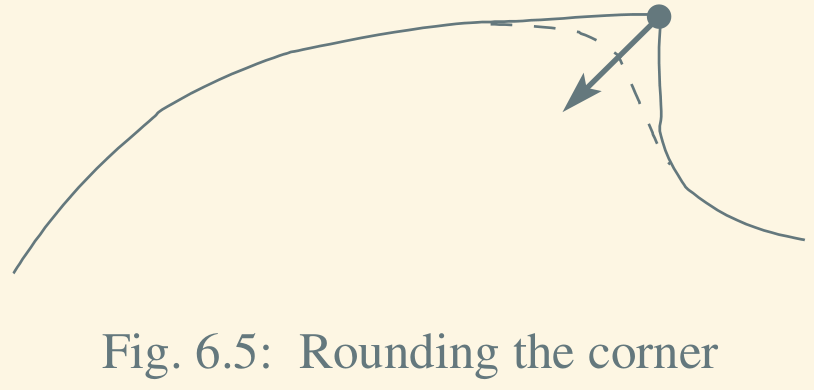
\includegraphics[width=0.3\textwidth]{fig3}
	\end{figure}
	so it would be nice to understand that precisely but \(\mathsf{OK}\).
\end{itemize}
\end{thing8}


\subsection{Duas geodésicas}
Mais um: 

\begin{thing4}{Exercício 8}[Curvas minimizantes]\label{exer:8}\leavevmode
\begin{enumerate}[label=(\alph*)]
	\item[(b)] Suponha que \(\gamma,\sigma:[0,2] \to M\) são geodésicas distintas e satisfazem: \(\gamma(0)=\sigma(0):=p\), \(\gamma(1)=\sigma(1):=q\), \(\gamma\) e \(\sigma\) realizam a distância entre \(p\) e \(q\). Mostre que \(\gamma\) não realiza a distância entre \(p\) e \(\gamma(1+s)\) para nenhum \(s>0\).
\end{enumerate}
\end{thing4}

\begin{proof}\leavevmode
Argumentamos na monitoria que teriamos um problema de diferenciabilidade. Pela explicação dada em  \cite{ler} sobre a suavização de quinas, sabemos que as geodésicas devem ser suaves. Porém, que não poderia acontecer algo assim?
\begin{figure}[H]
	\centering
	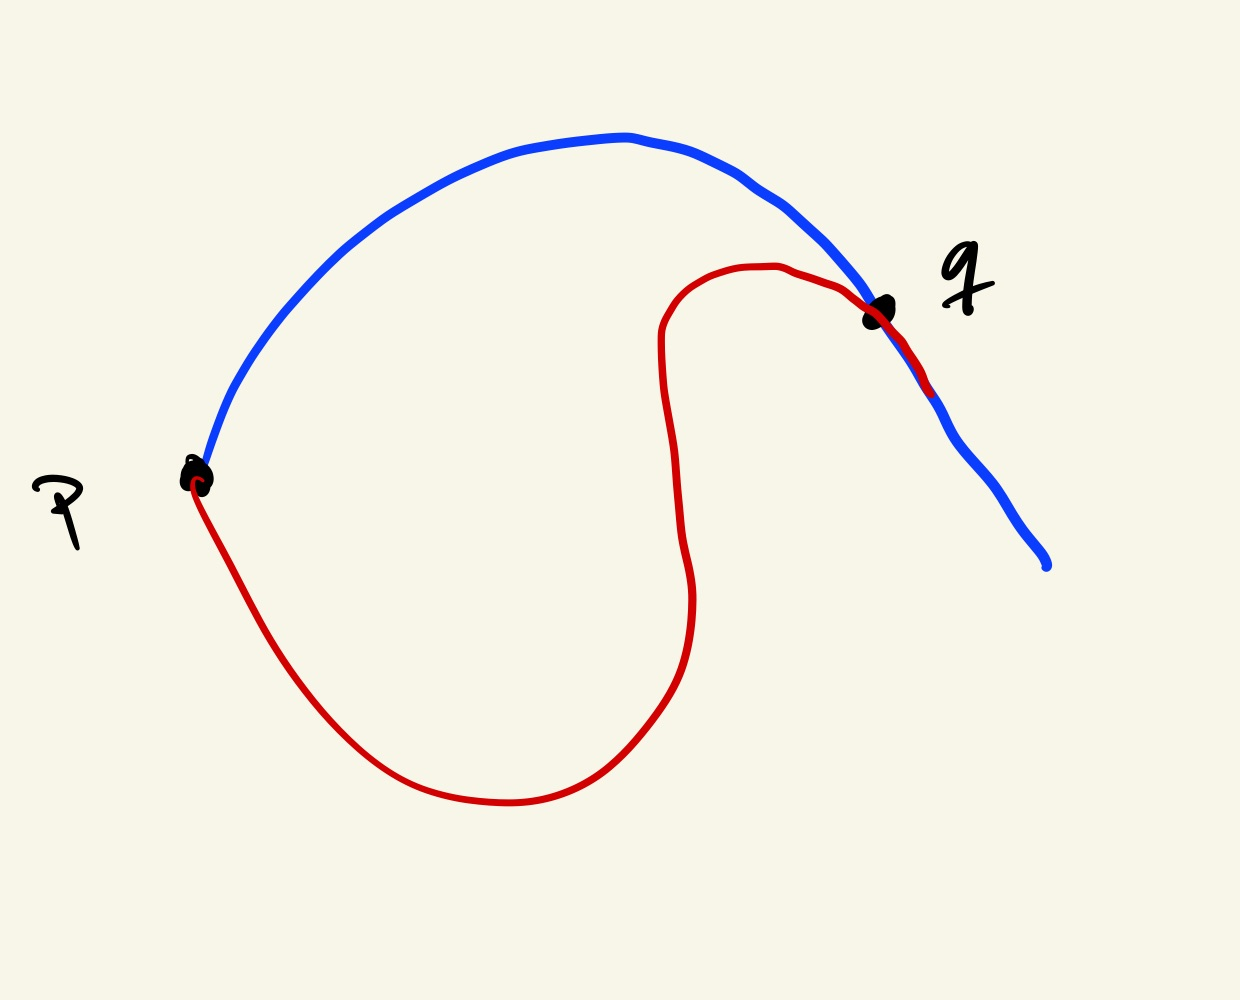
\includegraphics[width=.3\textwidth]{fig2}
\end{figure}
\end{proof}

\begin{exercise}\leavevmode
Show that for a bi-invariant metric on a Lie Group, it holds that \(\operatorname{exp}_e=\operatorname{exp}^G\).
\end{exercise}

\begin{proof}[Solution]\leavevmode
After delving into the abyss of definitions, I think it boils down to showing that \(\nabla_{X_v} X_v=0\), where \(v \in \mathfrak{g}\). So we have to use that the metric is bi-invariant. But it's not necessarily Levi-Civita connection…
\end{proof}

\clearpage
\section{Lista 1}

\subsection{Revisão}

\begin{thing4}{Exercício 1}\label{exer:1}\leavevmode
Dada uma subvariedade \(M \subseteq \tilde{M}\) uma subvariedade mergulhada e \(X \in \mathfrak{X}(M)\). Mostre que existe um aberto \(U \subset \tilde{M}\) contendo \(M\) e um campo \(\tilde{X} \in \mathfrak{X}(U)\) tal que \(\tilde{X}|_{M}=X\). Caso \(M\) seja subconjunto fechado de \(\tilde{M}\), prove que \(U\) pode ser tomado igual a \(\tilde{M}\). Se \(M\) não é subconjunto fechado de \(\tilde{M}\), pode não existir extensão de \(X\) definida em todo \(\tilde{M}\).
\end{thing4}

\begin{proof}[Solução]\leavevmode
Acho que a prova canônica é tomar coordenadas de subvariedade de \(M \subset \tilde{M}\), i.e. onde \(M\) está dada localmente como o lugar onde se anulam as últimas \(n-m\) funções coordenadas. 

Pegamos uma vizinhança rectificante \(U\) de \(X\) em \(p \in M\), i.e. \(X=\partial_1\) em \(U\). Daí pega para cada vetor normal a exponencial, que percorre pela geodésica um pouqinho. Isso da uma vizinhança em \(\tilde{M}\)…
\end{proof}

\begin{thing4}{Exercício 2}\label{exer:2}\leavevmode
	Seja \(f:M^n \to N^m\) um mapa suave. Os campos \(X \in \mathfrak{X}(M)\) e \(\tilde{X} \in \mathfrak{X}(N)\) são ditos \(f\)-relacionados se \(df_pX_p=\tilde{X}_{f(p)}\), \(\forall  p \in M\). Mostre que se os campos \(X,Y \in \mathfrak{X}(M)\) são, respetivamente, \(f\)-relacionados com \(\tilde{X},\tilde{Y} \in \mathfrak{X}(N)\) então \([X,Y]\) é \(f\)-relacionado com \([\tilde{X},\tilde{Y}]\).
\end{thing4}

\begin{proof}[Solução]\leavevmode
	\textbf{Intento 2.} \(s_1 \in \Gamma(\tau_N)\) está \textit{\textbf{\(f\)-relacionado}} com \(s \in \Gamma(\tau_M)\) se \(s=s_1\oplus s^\perp\) para algum \(s^\perp\in\nu\). Queremos ver que se \(s\overset{f}{\sim}s_1\) e \(t \overset{f}{\sim}t_1\), \([s,t]\overset{f}{\sim}[s_1,t_1]\), ou seja \([s,t]=[s_1,t_1]\oplus [s,t]^\perp\) onde \([s,t]^\perp\) é um vetor em \(\nu\) cuja cara não  é muito importante.
	\begin{align*}
		[s,t]&=[s_1\oplus s^\perp,t_1\oplus t^\perp]=[s_1,t_1]+\underbrace{[s_1,t^\perp]}_{=0}+\underbrace{[s^\perp,t_1]}_{=0}+\underbrace{[s^\perp,t^\perp]}_{\in \nu}
	\end{align*}
{\color{4}Falta un argumentín para ver que esos colchetes se anulan…}

\textbf{Intento 1 (incompleto).} Pegue \(p \in M\). Queremos ver que
\[(f_{*}[X,Y])_p\overset{\text{quero}}{=}[\tilde{X},\tilde{Y}]_{f(p)}.\]
Pegue \(g \in \mathcal{F}(N)\).
\begin{align*}
	[\tilde{X},\tilde{Y}]_{f(p)}&\overset{\operatorname{def}}{=}\tilde{X}_{f(p)}(\tilde{Y}g)-\tilde{Y}_{f(p)}(\tilde{X}g)\\
	&\overset{\operatorname{hip}}{=}f_{*,p}(X_p)(\tilde{Y}g)-f_{*,p}(Y_p)(\tilde{X}g)\\
	&=X_{p}\Big((\tilde{Y}g)\circ f\Big)-Y_p\Big((\tilde{X}g)\circ f\Big)\\
	&\overset{\operatorname{hip}}{=}X_p\Big(\big(f_{*,p}(Y)\big)g\circ f)\Big)-Y_p\Big(\big(f_{*,p}(X_p)\big)g \circ f\Big)\\
\end{align*}
\end{proof}

\begin{thing4}{Exercício 3}\label{exer:3}\leavevmode
Seja \(\pi:M \to N\) uma submersão sobrejetiva. Dado \(Y \in \mathfrak{X}(N)\), mostre que existe \(X \in \mathfrak{X}(M)\) tal que \(X\) é \(\pi\)-relacionado com \(Y\).
\end{thing4}
\begin{proof}[Solução]\leavevmode
O resultado segue de que \(\tau_M\cong\pi^*\tau_N\oplus \nu\), tomando \(X:=Y\oplus 0\).
\end{proof}

\begin{thing4}{Exercício 4}[Fibrado pullback]\label{exer:4}\leavevmode
Suponha que \(M^n\), \(N^m\) são variedades suaves, \(\pi:E \to M\) é um fibrado vetorial suave de posto \(k\) e \(f:N \to M\) é um mapa suave. Considere o espaço
\[f^*E=\{(p,e) \in N \times E:f(p)=\pi(e)\},\]
e \(\tilde{\pi}:E \to N\) a projeção na primeira coordenada. Mostre que \(f^*E\) tem uma estrutura de variedade suave de forma que a tripla \(\tilde{\pi}:f^*E\to N\) é um fibrado vetorial suave de posto \(k\).
\end{thing4}

\begin{proof}[Solução]\leavevmode
Para mostrar que \(\tilde{\pi}\) é um fibrado vetorial devemos dar trivializações locais. Pegue um ponto \(p \in M\) e uma vizinhança trivializante de \(E\) perto de \(f(p)\), i.e. um aberto \(U \ni f(p)\) e um difeomorfismo \(h:\pi^{-1}(U)\xrightarrow{\cong}U\times \mathbb{R}^k\). Pegue também um aberto \(V \ni p\) tal que \(f(V) \subset U\). Defina
\begin{align*}
	h_1: \tilde{\pi}^{-1}(V) &\longrightarrow V \times \mathbb{R}^k \\
	(q,v) &\longmapsto (q,\pi_2\circ h(f(q),v))
\end{align*}
Como estamos usando a estrutura de fibrado vetorial de \(E\), segue imediatamente a coleção de funções desse tipo formam um atlas trivializante de \(f^*E\).
\end{proof}

\subsection{Métricas Riemannianas}

\begin{thing4}{Exercício 6}\label{exer:6}\leavevmode
Seja \((N^n,g)\) uma variedade Riemanniana e \(M^m \subset N\) uma subvariedade mergulhada. Mostre que para todo \(p \in M\) existe uma vizinhança aberta \(U \subset N\) de \(p\) e campos vetoriais \(E_1,\ldots,E_n\) em \(U\) tal que \(E_1(q),\ldots,E_n(q)\) é uma base ortonormal de \(T_q N\) para todo \(q \in U\) e \(E_1(r),\ldots,E_m(r)\) são tangentes a \(M\) para todo \(r \in U \cap M\).
\end{thing4}

\begin{proof}[Solução]\leavevmode
\textbf{(Intento 1.)}Pegue \(p \in M\) e uma vizinhança aberta de \(U \subset N\) de \(p\) tal que \(U \cap M\) é suficientemente pequeno como para ter um marco ortonormal \(\{E_i\}_{i=1}^n\). Considere esses campos como campos tangentes a \(N\). Usando o exercício 1 podemos estender esses campos a uma vizinhança de \(U \subset N\). Aplicando Gram-Schmidt obtemos um marco ortonormal de  \(\mathfrak{X}(U)\).

\textbf{(Intento 2, \cite{mc} thm. 3.3, p. 36.)} Take orthonormal frames  \(\{E_i\}_{i=1}^m\subset\mathfrak{X}(U \cap M)\) and \(\{E_i'\}_{i=1}^n \subset \mathfrak{X}(U)\). Notice that the matrix \((E_i\cdot E_j')\) has rank \(m\) at \(p\). (I think that two orthonormal frames are related up to an orthogonal matrix.) Suppose that the first \(m\) columns are linearly independent at \(p\). Then there is an open neighbourhood \(V\) of \(p\) where the first \(m\) columns of this matrix are linearly independent. Then a slightly confusing part arguing that \(E_1,\ldots,E_m,E_{m+1}',\ldots,E_{n}'\) are linearly independent in \(V\). Then apply Gram-Schmidt. And that's it.

Then Milnor shows that this is a vector bundle called the \textit{\textbf{orthogonal bundle}}. The lance is that the orthonormal frame we have found gives the local trivialization. For a subbundle \(\xi \subset \eta\) define the fiber of the orthogonal complement of \(\xi\) by \(F_b(\xi^\perp):=F_b(\xi)^\perp\) with respect to the metric of \(\eta\). Define local trivializations by
\begin{align*}
	\overline{h}: \overline{\pi}^{-1}(U) &\longrightarrow U\times \mathbb{R}^{n-m} \\
	 \Big(q,\sum x_iE_i\Big)&\longmapsto (q,x_{m+1},\ldots,x_m)
\end{align*}

\end{proof}

\begin{thing4}{Definição 1}\label{def:1}\leavevmode
Sejam \((M^m,g_M)\) e \((N^n,g_N)\) variedades Riemannianas. Seja \(F:M \to N\) uma submersão. Dizemos que \(F\) é uma \textit{\textbf{submersão Riemanniana}} quando para todo \(p \in M\), \(DF: \ker (DF)^\perp\to T_{F(p)}N\) é uma isometría linear. Em outras palavras, sempre que \(v, w \in T_pM\) são perpendiculares ao núcleo de \(DF\), vale
\[g_M(v,w)=g_N(DF(v),DF(w)).\]
\end{thing4}

\begin{thing4}{Exercício 7}\label{exer:7}\leavevmode
Seja \((M^n,g)\) uma variedade Riemanniana. Suponha que existe um grupo de Lie \(G\) agindo por isometrias em \((M,g)\) de tal forma que \(M/G\) admite uma estrutura de variedade suave, onde a projeção \(\pi:M \to M/G\) é uma submersão. Mostre que existe uma métrica Riemanniana \(\overline{g}\) em \(M/G\) tal que \(\pi:(M,g) \to (M/G,\overline{g})\) é uma submersão Riemanniana.
\end{thing4}
\begin{proof}[Solução]\leavevmode
	\textbf{(Seguindo notação e ideias de \cite{mc}.)} Fazemos assim para definir a métrica em \(G/M\). Primeiro lembre que \(\tau_{G/M} \cong \pi^*\tau_{M/G}\). Considere o fibrado \(\nu\) normal a \(\pi^*\tau_{M/G}\), que é um fibrado sobre \(M\) satisfazendo \(\pi^*\tau_{G/M}\oplus \nu\cong\tau_M\). Então qualquer vetor tangente a \(M/G\) pode ser pensado como um vetor tangente a \(M\) se anulamos a parte normal dele, mostrando que podemos usar a mesma métrica em \(M\) para introduzir uma métrica em \(G/M\).

	Para resolver o exercício devemos analisar como age \(\pi_*\) em \(\tau_M\) quando este es visto como soma direita \(\pi^*\oplus \nu\): \(\pi_*(v_1 \oplus v^\perp)=v_1\). Daí segue trivialmente que \(\ker \pi:=\kappa\subset\nu\). Conversamente se \(v_1 \oplus v^\perp \in \kappa\), fazemos para \(w \in \pi^*\)
	\begin{align*}
	(v_1 \oplus  v^\perp)\cdot w&=v_1 \cdot w+\cancelto{0}{v^\perp\cdot w}=\pi_*v_1\cdot\pi_*w=0.
\end{align*}
Então \(\kappa=\nu\), então \(\kappa^\perp\cong\pi^*\cong\tau_{M/G}\) isometricamente.

	\textbf{Intento 1 (errado).} Defina a seguinte métrica em \(M/G\):
\[g_{M/G}:=g_M|_{\pi^*\tau_{M/G}}\]
i.e. a restrição da métrica em \(M\) ao fibrado pullback de \(\tau_{M/G}:=T(G/M)\), que sabemos que é isomorfo (como fibrado) a \(\tau_{M/G}\).

Para ver que \(\pi:M\to M/G\) é uma submersão Riemanniana devemos mostrar que o complemento ortogonal de \(\kappa_\pi:=\ker(\pi)\) é isomorfo (como fibrado Riemanniano, i.e. isométrico como fibrado) a \(\tau_{M/G}\).

Como \(M\) é Riemanniana, o fibrado pullback tem um complemento ortogonal \((\pi^*\tau_{M/G})^\perp := \nu\). Basta mostrar que \(\nu \cong\kappa\) isometricamente.



\end{proof}

\section{Lista 2}

\begin{thing4}{Exercício 1}\label{exer:1}\leavevmode
Mostre que todo fibrado vetorial admite uma conexão.
\end{thing4}

\begin{thing4}{Exercício 3}\label{exer:3}\leavevmode
Exercício 2 do Capítulo 2 do livro do professor Manfredo:

Sejam \(X\) e \(Y\) campos de vetores numa variedade Riemanniana \(M\). Sejam \(p \in M\) e \(\gamma: I \to M\) uma curva integral de \(X\) por \(p\), i.e. \(\gamma(t_0)=p\) e \(\frac{d\gamma}{dt}=X(\gamma(t))\). Prove que a conexão Riemanniana de  \(M\) é
\begin{equation}\label{eq:1}(\nabla_XY)(p)= \frac{d}{dt}\Big(P^{-1}_{\gamma,t_0,t}(Y(\gamma(t)))\Big)\Big|_{t=t_0}\end{equation}
onde \(P_{\gamma,t_0,t}:T_{\gamma(t_0)M\to T_{\gamma(t)}M}\) é o transporte paralelo ao longo de \(\gamma\) de \(t_0\) a \(t\).
\end{thing4}

\begin{proof}[Solução]\leavevmode
Primeiro devemos escrever o lado direito da  \cref{eq:1} em termos do fibrado pullback ao longo de \(\gamma\):
\[\frac{d}{dt}\Big(P^{-1}_{\gamma,t_0,t}(Y(\gamma(t)))\Big)\Big|_{t=t_0} \leftrightsquigarrow \nabla^\gamma_{\frac{d}{dt}}\]

\end{proof}


\clearpage
\begin{minipage}{\textwidth}
	\begin{minipage}{1\textwidth}
		{\small Prof. Luis Florit\hfill Daniel González Casanova Azuela}
		
		{\small Monitor. Ivan Miranda\hfill\href{https://github.com/danimalabares/rg}{github.com/danimalabares/rg}}
	\end{minipage}
\end{minipage}\vspace{.2cm}\hrule

\vspace{10pt}
{\huge Lista 3}
\addcontentsline{toc}{section}{Lista 3}

\begin{thing4}{Exercício 4}\label{exer:4}\leavevmode
Exemplo: esfera.
\begin{enumerate}[label=(\alph*)]
\item Determine as geodésicas da esfera \(\mathbb{S}^n\) com sua métrica canônica.
\item Determine o grupo de isometrias da esfera \(\mathbb{S}^n\) com sua métrica canônica.
\end{enumerate}
\end{thing4}

\begin{proof}[Solution]\leavevmode
\begin{enumerate}[label=(\alph*)]
\item \textbf{Ideia essencial.} Suponha que \(\gamma:I \to \mathbb{S}^n \subset \mathbb{R}^{n+1}\) é uma geodésica. Podemos pensar que \(\gamma':I \to T\mathbb{S}^n \subset T\mathbb{R}^{n+1}=\mathbb{R}^{n+1}\) e analogamente \(\gamma'':I \to \mathbb{R}^{n+1}\). Espaço tangente à esfera é perpendicular ao vetor posição, i.e. \(\gamma \perp \gamma'\). Também \(\gamma'' \perp \gamma'\); isso é porque \(\gamma''=(\gamma'')^{\top}+(\gamma'')^{\perp}\), e como \(\gamma\) é geodésica sabemos que \((\gamma'')^{\top}=0\). Por fim, \(\gamma''=\lambda \gamma\), então concluímos que \(\gamma\) está dada por senos e cosenos.
\vspace{1em}

	Para escrever isso formalmente precisamos de uma expressão experta para \(\gamma\).  Em \cite{ler} Prop. 5.27 achamos inspiração: damos a volta ao problema e começamos propondo uma curva que vai acabar sendo geodésica. Pegue um ponto \(p \in \mathbb{S}^n\) e um vetor unitário \(v \in T_p\mathbb{S}^n\). Considere
	\[\gamma(t)=\cos t p+\sin t v\]
Derivando como uma simples curva em \(\mathbb{R}^{n+1}\), vemos que \(\gamma''=-\gamma\), o que significa que \((\gamma'')^{\top}=0\), i.e. \(\gamma\) é uma geodésica de \(\mathbb{S}^n\). Mais precisamente,
\[\gamma''(t)=\Big(\nabla_{\frac{d}{dt}}^{i \circ \gamma}\gamma'\Big)_t \in (i \circ \gamma)^*T\mathbb{R}^{n+1}\cong \gamma ^* (T\mathbb{S}^n \oplus N)\]
não tem componente tangente, e portanto
 \[0=\nabla_{\frac{d}{dt}}^{\gamma}\gamma' \in \gamma^* T\mathbb{S}^n.\]
Sendo essa uma geodésica partindo de um ponto arbitrário numa direção arbitrária, concluimos por unicidade das geodésicas e \textit{rescaling lemma} que todas as geodésicas de \(\mathbb{S}^n\) são como \(\gamma\).

Note que a geodésica \(\gamma\) é uma parametrização do círculo unitário no plano gerado pelos vetores \(p\) e \(v\), i.e. um círculo máximo. Em conclusão, as geodésicas são os círculos máximos de \(\mathbb{S}^n\).

\item Afirmo que \(\operatorname{Isom}\mathbb{S}^n=\mathsf{O}(n+1)\overset{\operatorname{def}}{=}\{A \in \mathsf{GL}(n+1):A A^{\mathbf{T}}=\operatorname{Id}\}\). É claro que \(\mathsf{O}(n+1)\subset \operatorname{Isom}\mathbb{S}^{n}\), pois as transformações \(A \in \mathsf{O}(n+1)\) preservam o produto interno euclideano:
\begin{align*}
&A A^{\mathbf{T}}=\operatorname{Id}\iff \sum_k A_{ik}A_{jk}=\delta_{ij} \iff Ae_i\cdot Ae_j=\delta_{ij}\\ &\iff Av\cdot Aw=A\left( v^ie_i\right) \cdot A\left( w^je_j\right) =v^iw^j e_i\cdot e_j=v\cdot w.
\end{align*}
	Para ver que \(\operatorname{Isom}\mathbb{S}^n \subset\mathsf{O}(n+1)\) suponha que \(A:\mathbb{S}^n \to \mathbb{S}^n\) é uma isometria. Vamos mostrar que \(A\) é a restrição de uma função \(\tilde{A} \in \mathsf{O}(n+1)\). Defina
	\begin{align*}
		\tilde{A}: \mathbb{R}^{n+1} &\longrightarrow \mathbb{R}^{n+1} \\
		(r,\theta) &\longmapsto rA(1,\theta)\\
		0&\longmapsto 0
	\end{align*}
	Se mostramos que \(\tilde{A}\) é uma isometria linear, é claro que ela é um elemento de \(\mathsf{O}(n+1)\) pela conta anterior. De fato, basta mostrar que \(\tilde{A}\) é uma isometria, pois toda isometria de espaços de Banach que fixa a origem é linear (\cite{braga} Teo. 7.11).

	Para ver que \(\tilde{A}\) é uma isometria de \(\mathbb{R}^{n+1}\), \textbf{afirmo}  que a distância de \(p\) a \(q\) está totalmente determinada pelas normas  \(\|p\|\) e \(\|q\|\), e pela distancia esférica entre  \(\frac{p}{\|p\|}\) e \(\frac{q}{\|q\|}\). Note que essa afirmação é na verdade um problema de geometria plana, pois todas essas quantidades podem ser descritas dentro do único plano que contém \(0\), \(p\) e \(q\).
\begin{figure}[H]
	\centering
	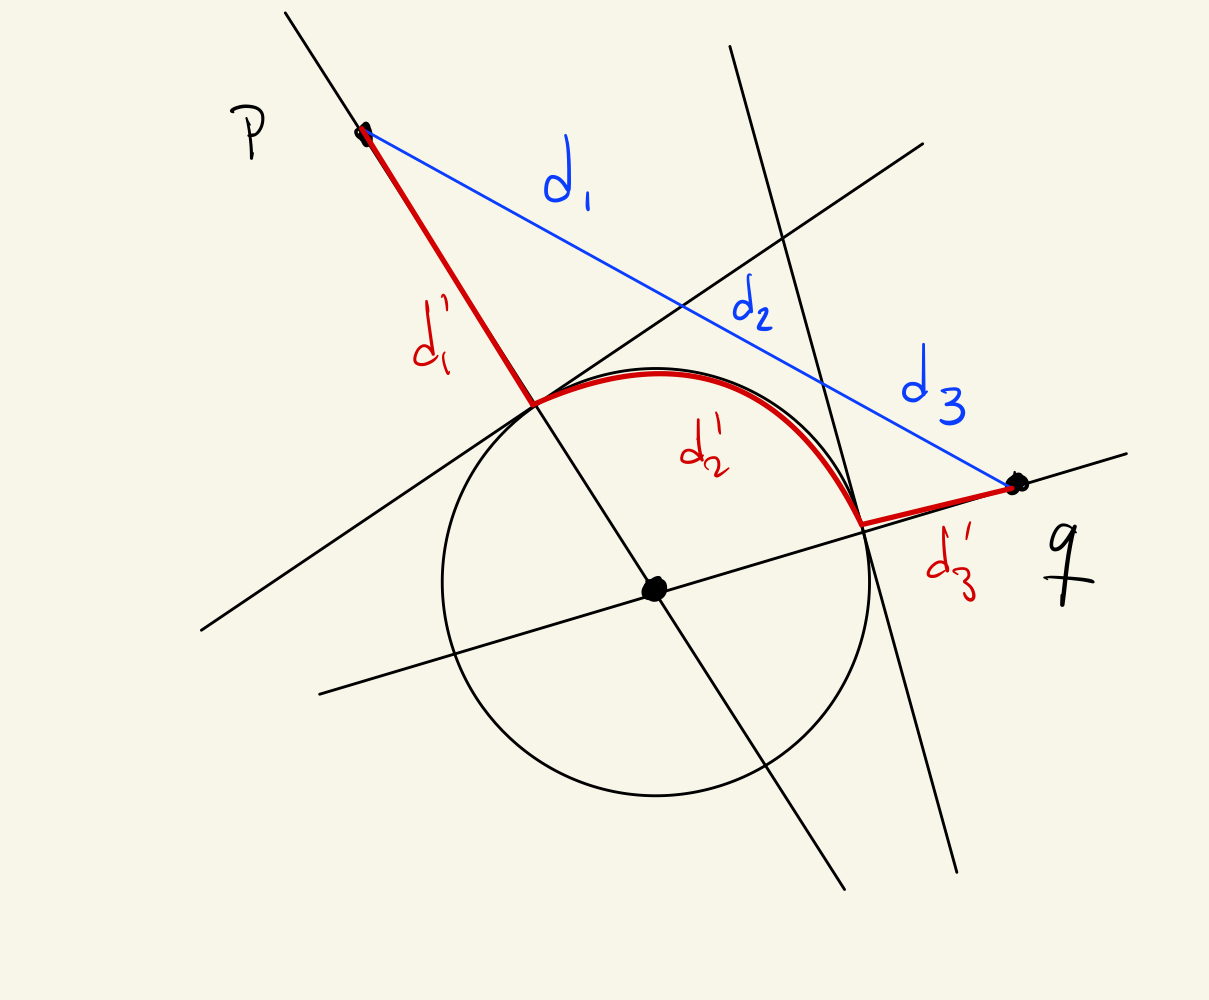
\includegraphics[width=0.6\textwidth]{fig1}
	\caption{Intento de prova}
\end{figure}

	Acabou que essa afirmação é simplesmente a lei dos cosenos, já que a distância esférica entre \(\frac{p}{\|p\|}\) e \(\frac{q}{\|q\|}\) é exatamente o angulo entre \(p\) e \(q\) (poque essa distância é um segmento de círculo máximo!):
	\[\text{lei dos cosenos:} \qquad d(p,q)^2=\|p\|^2+\|q\|^2-2\|p\|\|q\| \cos \angle(p,q) \]

Em fim, \(\tilde{A}\) é uma isometria porque \(d_{\mathbb{R}^{n+1}}(p,q)=d_{\mathbb{R}^{n+1}}(\tilde{A}p,\tilde{A}q)\) pelo argumento anterior. 
\end{enumerate}
\end{proof}

\begin{thing4}{Exercício 12}\label{exer:12}\leavevmode
Seja \((G,g)\) um grupo de Lie munido de uma métrica bi-invatiante e \(\nabla\) sua conexão de Levi-Civita.
\begin{enumerate}[label=(\alph*)]
\item Mostre que
	\[\nabla_uv=\frac{1}{2}[u,v],\]
	para cada \(u,v \in \mathfrak{g} \subset \mathfrak{X}(G)\).
\item Seja \(\overline{\nabla}\) uma conexão agim simétrica em \(G\). Mostre que \(\overline{\nabla}=\nabla\) se e somente se \(\overline{\nabla}_uu=0\) para todo \(u \in \mathfrak{g}\).
\end{enumerate}
\end{thing4}


\begin{proof}[Solution]\leavevmode
\begin{enumerate}[label=(\alph*)]
\item Como \(\nabla\) é Levi-Civita, temos Koszul, i.e. \(\forall  u,v,w \in \mathfrak{g}\),
	\begin{align*}
	2\left<\nabla_uv,w\right>&=u\left<v,w\right>+v\left<u,w\right>-w\left<u,v\right>\\
				 & -\left<u,[v,w]\right>+\left<v,[w,u]\right>+\left<w,[u,v]\right>
	\end{align*}
	Como \(\left<\cdot,\cdot\right>\) é invariante à esquerda, é constante quando avaliamos em elementos de \(\mathfrak{g}\), e portanto os primeiros três termos se anulam. Então o exercício acaba quando mostramos que
	\[\left<v,[w,u]\right>=\left<u,[v,w]\right>=-\left<u,[w,v]\right>.\]
	Seguindo \cite{doc}, p. 45., a ideia é usar o fluxo \(\varphi:\mathbb{R} \times G\to G\) de \(w\) para expressar o colchete de Lie. Primeiro precisamos de

	\begin{claim}\leavevmode
	O fluxo \(\varphi\) de um campo invariante à esquerda \(w\) comuta com a traslação à esquerda, i.e.,
	\[\varphi_t(e)\circ L_h = L_h \circ \varphi_t(e)\qquad \forall t\in \mathbb{R} \forall h \in G.\]
	\end{claim}
	\begin{proof}[Prova da afirmação]\leavevmode
Derivamos de ambos lados. Por um lado,
\begin{align*}
\frac{d}{dt}\Big|_{t=0}\varphi_t(e) \circ L_h=\frac{d}{dt}\Big|_{t=0}\varphi_t(h)&=v_h\end{align*}
Por outro lado,
\[\frac{d}{dt}\Big|_{t=0}L_h \circ \varphi_t(e)=(L_h)_{*,\varphi_t(e)}\frac{d}{dt}\Big|_{t=0}\varphi_t(e)=(L_h)_{*,e}v_e=v_h.\]
Por unicidade das soluções de EDOs, acabou.
	\end{proof}
Então repare:
\[\varphi_t(h)=(\varphi_t\circ L_h)(e)=(L_h \circ \varphi_t)(e)=h\varphi_t(e)=R_{\varphi_t(e)}h,\]
ou seja, qualquer curva integral de \(w\) é simplesmente a curva integral que passa por \(e\) trasladada.

Agora lembre que o colchete de Lie pode ser expressado como
\[[w,v]_e=\frac{d}{dt}\Big|_{t=0}\Big(\varphi_{-t}\Big)_{*,\varphi_t(e)}v_{\varphi_t(e)}.\]
(Onde fixamos o parámetro \(-t\) e deixamos livre o outro para ver \(\varphi_{-t}\) como um difeomorfismo de \(G\).)

Juntando com a discussão anterior obtemos
\[[w,v]_e=\frac{d}{dt}\Big|_{t=0}\Big(R_{\varphi_{-t}(e)}\Big)_{*,\varphi_t(e)}v_{\varphi_t(e)}.\]
Agora repare: como a métrica é bi-invariante,
\begin{align*}
\left<u,v\right>&=\left<\Big(R_{\varphi_{-t}(e)}\Big)_{*,\varphi_t(e)}\Big(L_{\varphi_{t}(e)}\Big)_{*,e}u_{e},\Big(R_{\varphi_{-t}(e)}\Big)_{*,\varphi_t(e)}\Big(L_{\varphi_{t}(e)}\Big)_{*,e}v_{e}\right>\\
&=\left<\Big(R_{\varphi_{-t}(e)}\Big)_{*,\varphi_t(e)}u_{\varphi_t(e)},\Big(R_{\varphi_{-t}(e)}\Big)_{*,\varphi_t(e)}v_{\varphi_t(e)}\right>
\end{align*}
Agora derivemos como funções de \(t\) (dentro de \(T_eG\), i.e. não precisamos derivada covariante), e avaliemos em  \(t=0\). (Note que quando avaliamos em  \(t=0\) o factor que não derivamos não muda---estamos trasladando à direita e à esquerda por \(\varphi_0(e)\)!) Obtemos:
\begin{align*}
0&=\frac{d}{dt}\Big|_{t=0}\left<\Big(R_{\varphi_{-t}(e)}\Big)_{*,\varphi_t(e)}u_{\varphi_t(e)},\Big(R_{\varphi_{-t}(e)}\Big)_{*,\varphi_t(e)}v_{\varphi_t(e)}\right>\\
 &=\left<\frac{d}{dt}\Big|_{t=0}\Big(R_{\varphi_{-t}(e)}\Big)_{*,\varphi_t(e)}u_{\varphi_t(e)},\left[\Big(R_{\varphi_{-t}(e)}\Big)_{*,\varphi_t(e)}v_{\varphi_t(e)}\right]_{t=0}\right>\\
&+\left<\left[\Big(R_{\varphi_{-t}(e)}\Big)_{*,\varphi_t(e)}u_{\varphi_t(e)}\right]_{t=0},\frac{d}{dt}\Big|_{t=0}\Big(R_{\varphi_{-t}(e)}\Big)_{*,\varphi_t(e)}v_{\varphi_t(e)}\right>\\
&=\left<[w,u]_e,v_e\right>+\left<u_e,[w,v]_e\right>.
\end{align*}
\end{enumerate}

\item Pelo inciso (a), é claro que se  \(\overline{\nabla}=\nabla\), \(\overline{\nabla}_u u=0\). Para a implicação contrária, vejamos que
	\[\overline{\nabla}_uv=\frac{1}{2}[u,v],\qquad u,v \in \mathfrak{g}\]
	que é conveniente porque sabemos que isso é igual a \(\nabla_uv\) pelo inciso (a). É só fazer:
	\[0=\overline{\nabla}_{u+v}u+v=\cancelto{0}{\overline{\nabla}_u u}+\overline{\nabla}_uv+\overline{\nabla}_vu+\cancelto{0}{\overline{\nabla}_vv}\]
Lembre que \(\overline{\nabla}\) é simétrica, i.e. \(\overline{\nabla}_uv-\overline{\nabla}_vu=[u,v]\). Somando com a equação anterior:
\begin{align*}
	\overline{\nabla}_uv-\overline{\nabla}_vu+\overline{\nabla}_uv+\overline{\nabla}_vu=[u,v]
\end{align*}
como queríamos. Para concluir é só ver que \(\nabla\) e \(\overline{\nabla}\) também coincidem em campos vetoriais que não são invariantes à esquerda. Então pegue uma base \(\{u_i\}\subset \mathfrak{g}\) e dois campos \(X=X^iu_i\),\(Y=Y^ju_j\) quaisquer. Então:
\begin{align*}
\overline{\nabla}_XY&=\overline{\nabla}_{X^iu_i}Y^ju_j=X^iu_iY_ju_j+Y^j\overline{\nabla}_{u_i}u_j=X^iu_iY_ju_j+Y^j\nabla_{u_i}u_j=\nabla_XY.
\end{align*}
\begin{question}\leavevmode
Tem algum argumento super simples para argumentar essa última parte sem pegar uma base de \(\mathfrak{g}\)?
\end{question}
\end{proof}

\begin{thing4}{Exercício 13}[Exercício 3, Cap. III, \cite{doc}]\label{exer:13}\leavevmode
Sejam \(G\) um grupo de Lie,  \(\mathfrak{g}\) sua álgebra de Lie, e \(X \in \mathfrak{g}\). As trajetórias de \(X\) determinam uma aplicação \(\varphi:(-\varepsilon,\varepsilon)\to G\) com \(\varphi(0)=e\), \(\varphi'(t)=X(\varphi(t))\).
\begin{enumerate}[label=(\alph*)]
\item Prove que \(\varphi(t)\) está definida para todo \(t \in \mathbb{R}\) e que \(\varphi(t+s)=\varphi(t)\cdot\varphi(s)\), (\(\varphi:\mathbb{R} \to G\) é então chamado um \textit{\textbf{subgrupo a 1-parâmetro de \(G\)}}.
\item Prove que se \(G\) tem uma métrica bi-invariante \(\left<\cdot,\cdot\right>\) então as geodésicas de \(G\) que partem de \(e\) são os subgrupos a 1-parâmetro de \(G\).
\end{enumerate}
\end{thing4}

\begin{proof}[Solution]\leavevmode
\begin{enumerate}[label=(\alph*)]
\item Lembre que no exercício anterior mostramos que
	\[\varphi_t(h)=R_{\varphi_t(e)}(h)=h\cdot \varphi_t(e),\qquad \forall t \in (-\varepsilon,\varepsilon),\;\forall h \in G.\]
	Fixe um \(t_0 \in (-\varepsilon,\varepsilon)\) e pegue \(h=\varphi_{t_0}(e)^{-1}\). Obtemos que
	\[\varphi_t(\varphi_{t_0}(e)^{-1})=\varphi_{t_0}(e)^{-1}\varphi_t(e).\]
Ou seja,  \(\varphi_{t_0}(e)^{-1}\varphi_t(e)\) é uma curva integral de \(X\) que passa por \(e\) no tempo \(t=t_0\). Como também \(\varphi_{t-t_0}(e)\) é uma curva integral de \(X\) que passa por \(e\) no tempo \(t=t_0\), por unicidade de EDOs obtemos
\begin{equation}\label{eq:2}
\varphi_{t_0}(e)^{-1}\varphi_t(e)=\varphi_{t-t_0}(e)
\end{equation}
Avaliando o lado esquerdo em \(t'=t-t_0\), do lado direito chegamos até \(\varphi_{t-2t_0}(e)\). Repetindo esse processo cobrimos todo \(\mathbb{R}\).

Para confirmar a segunda propriedade avaliamos \cref{eq:2} em \(t=0\) para obter \(\varphi_{t_0}(e)^{-1}=\varphi_{-t_0}(e)\). Para concluir pegue  \(t,s \in \mathbb{R}\) quaisquer e escreva:
\[\varphi_{t+s}(e)=\varphi_{t-(-s)}(e)=\varphi_{-s}^{-1}\varphi_t(e)=\varphi_s(e)\varphi_t(e).\]

\item Pegue \(X \in \mathfrak{g}\) e considere a curva integral que passa por \(e\), \(\varphi\). Pelo exercício anterior,
\[0=\nabla_X X=\nabla_{\varphi_*\frac{d}{dt}}X=\nabla_{\frac{d}{dt}}^\varphi X \circ \varphi=\nabla_{\varphi'}\varphi'\]
Então as curvas integrais de \(X\) que passam por \(e\) são geodésicas. Como isso é para qualquer vetor em \(\mathfrak{g}\), por unicidade das soluções a EDOs, acabou.
\end{enumerate}
\end{proof}

\clearpage
\begin{thing4}{Exercício 14}\label{exer:14}\leavevmode
Dada uma variedade Riemanniana \((M^n,g)\) denotamos por \(d_g\) a distância induzida por \(g\).
\begin{enumerate}[label=(\alph*)]
\item Sejam \(g,h\) duas métricas Riemannianas em \(M^n\). Mostre que se \(d_g=d_h\) então \(g=h\).
\item Seja \((M,g)\) uma variedade Riemanniana e \(F:M \to M\) um difeomorfismo. Mostre que \(F\) é uma isometria se e somente se \(d_g(F(\cdot),F(\cdot))=d_g(\cdot,\cdot)\).
\end{enumerate}
\end{thing4}

\begin{proof}\leavevmode
\begin{enumerate}[label=(\alph*)]
\item  Prova por contrapositiva.
	\begin{claim}\leavevmode
	Se \(g \neq h\), existem um aberto \(U\subset M\) e um marco \(\{E_i\}\subset \mathfrak{X}(U)\) tais que
	\[g(E_{i_0},E_{i_0}) \neq  h(E_{i_0},E_{i_0})\qquad \text{para algum } i_0\in \{1,\ldots,n\}.\]
	\end{claim}
	\begin{proof}[Prova da afirmação.]\leavevmode
	Se \(g(E_i,E_i)=h(E_i,E_i)\) para todo marco em todo aberto de \(M\), é claro que \[g(X,Y)=g(X^iE_i,Y^jE_j)=X^iY^jg(E_i,E_j)=h(X,Y)\]
para quaisquer \(X,Y \in \mathfrak{X}(M)\).
	\end{proof}
	Então pegue um marco \(\{E_i\} \in \mathfrak{X}(U)\) tal que \(g(E_{i_0},E_{i_0})\neq h(E_{i_0},E_{i_0})\) em \(U\). Sendo a diferença dessas quantidades uma função distinta da constante zero, podemos supô-la estritamente positiva dentro de \(U\). Pegue \(p \in U\) e uma vizinhança geodésica contendo \(p\), que renomeamos \(U\) por simplicidade. Dentro de uma vizinhança geodésica, a distância de \(p\) aos outros pontos dentro de \(U\) está realizada por geodésicas, então podemos pegar \(q \in U\) e \(\gamma\) geodésica ligando \(p\) e \(q\).

	Considere uma extensão de \(\gamma'\in \mathfrak{X}_\gamma\) dentro de \(U\), digamos \(G=G^iE_i\). Então:
	\begin{align*}
	d_g(p,q)&=\int_a^b g(G^iE_i,G^iE_i) \circ \gamma dt=\int_a^b (G^i \circ \gamma)^2g(E_i,E_i) \circ \gamma dt\\&\neq \int_a^b(G^i \circ \gamma)^2 h(E_i,E_i)\circ \gamma dt = d_h(p,q).
	\end{align*}

\item Primeiro suponha que \(F^*d_g=d_g\). Para mostrar que \(F\) é uma isometria usamos o inciso anterior: consideramos as métricas \(g\) e \(F^*g\) em \(M\). Basta mostrar que \(d_g=d_{F^*g}\). Por um tempo pensei que era para usar um câmbio de variáveis, mas acabei pensando assim: Pegue uma curva \(\gamma\) ligando \(p\) e \(q\). Note que
	\[\underbrace{\int_a^bF^* g(\gamma'(t),\gamma'(t))dt}_{\ell(\text{curva de \(p\) a \(q\)} )}=\underbrace{\int_a^bg(F_{*,\gamma(t)}\gamma'(t),F_{*,\gamma(t)}\gamma'(t))dt}_{\ell(\text{curva de \(F(p)\) a \(F(q)\)} )}\]
Ou seja, do lado esquerdo estamos medindo o comprimento (respeito à métrica \(F^*g\)) de uma curva ligando \(p\) a \(q\), enquanto que do lado direito estamos medindo o comprimento (respeito à métrica \(g\)) da curva \(F\circ \gamma\), que liga \(F(p)\) a \(F(q)\).

Pegando o ínfimo de ambas quantidades, concluímos que a distância \(d_{F^*g}\) coincide com a distância \(F^*d_g\), que por hipótese é igual a \(d_g\). A implicação contrária também fica clara: supondo que \(F^*g=g\), levando em conta a igualdade das integrais acima e pegando o ínfimo, concluímos que \(F^*d_g=d_g\).
\end{enumerate}
\end{proof}

\begin{thing4}{Exercício 15}\label{exer:15}\leavevmode
Suponha que \((M^n,g)\) é uma variedade Riemanniana conexa.
\begin{enumerate}[label=(\alph*)]
\item \((M,g)\) simétrica \(\implies\) \((M,g)\) homogênea.
\item \((M,g)\) 2-homogênea \(\implies\) \((M,g)\) isotrópica.
\end{enumerate}
\end{thing4}

\begin{proof}[Solution]\leavevmode
\begin{enumerate}[label=(\alph*)]
	\item \textbf{Ideia.} Pegamos dois pontos \(q, q' \in M\). Para usar que \(M\) é simétrica buscamos o ``ponto meio". Esse deve ser \(p\in M\) que esteja no meio do caminho de uma curva minimizante \(\gamma\) ligando \(q\) e \(q'\). Daí, pegamos \(F \in \operatorname{Iso}_p:=\{\text{ isometrias de \(M\) que fixam \(p\)}\}\) com a propriedade de que \(d_pF=-\operatorname{Id}\). Daí devemos provar que \(F\) preserva \(\gamma\) e não fixa \(q\). Daí, só existem dois pontos em \(\gamma\) que guardam a mesma distância com \(p\): \(q\) e \(q'\). Como  \(F(q)\neq  q\) também guarda essa distância, concluímos que \(F(q)=q'\).

Infelizmente fui incapaz de levar minha ideia até uma prova sem ajuda externa. Primeiramente me pareceu improvável a possibilidade de construir a geodésica minimizante (pode não existir para variedades não completas; mostrar que a propriedade de simetria implica a existência de curvas minimizantes parecia muito forte).

\begin{conjecture}
	 Para quaisquer \(q,q' \in M\) existe uma curva minimizante \(\gamma\) ligando \(q\) e \(q'\).
\end{conjecture}
	Supondo que existe \(\gamma\), podemos pegar \(F \in \operatorname{Iso}_p\) tal que \(d_pF=-\operatorname{Id}\) onde \(p\) é ponto meio sobre \(\gamma\) respeito \(q\) e \(q'\).

	Tentei mostrar que \(F\) preserva \(\gamma\) perto de \(p\) usando um marco geodésico, onde a geodésicas são curvas integrais de linhas, mas depois descobri que minha prova estava errada (pois \(dF\) só age como \(-\operatorname{Id}\) em \(p\)):
	\begin{thing8}{Afirmação}\leavevmode
	Perto de \(p\), \(F(\gamma(t)) \in \operatorname{img} \gamma\).
	\end{thing8}
	\begin{proof}[Prova da afirmação]\leavevmode
	Pegue coordenadas geodésicas centradas em \(p\), de modo que as curvas minimizantes como \(\gamma\) são imagens de retas em \(T_pM\) baixo a exponencial. Agora derivamos: \(F \circ \gamma\):
	\[\frac{d}{dt}\Big|_{t}F \circ \gamma=F_{*,\gamma(t)}\gamma'(t)=-\gamma'(t).\]
	Portanto, a derivada da curva \(F \circ \gamma\) coincide com a derivada de \(\gamma\). Por unicidade de soluções de EDOs, concluímos que \(F \circ \gamma(t) \in \operatorname{img} \gamma\) dentro desta bola geodésica.
	\end{proof}
Depois desse ponto comecei a buscar ajuda em livros, internet e ChatGPT. Rapidamente reparei que minhas ideias eram boas, e consegui:
	\begin{proof}[Prova da afirmação reforçada]\leavevmode
	Pegue coordenadas geodésicas centradas em \(p\), de modo que as curvas minimizantes como \(\gamma\) são imagens de retas em \(T_pM\) baixo a exponencial. Agora derivamos: \(F \circ \gamma\) em \(t=0\) (supondo que \(\gamma(0)=p\)):
	\[\frac{d}{dt}\Big|_{t=0}F \circ \gamma=F_{*,p}\gamma'(0)=-\gamma'(0).\]
	Portanto, a derivada da curva \((F \circ \gamma)(t)\) coincide com a derivada de \(\gamma(-t)\). Por unicidade de soluções de EDOs, concluímos que \(F \circ \gamma(t) \in \operatorname{img} \gamma\) dentro desta bola geodésica.
	\end{proof}
Seguindo com esse raciocínio, \(F \circ \gamma\) é uma curva definida em todo o domínio de \(\gamma\), e portanto deve coincidir com \(\gamma(-t)\) ao longo desse domínio. Ou seja, \(F \circ \gamma\) é \(\gamma\) percorrida em sentido oposto. Isso significa, por definição de \(p\) como ponto meio, e desde que supomos que \(\gamma(0)=p\), que, se \(\gamma(t_0)=q\), necessariamente \(q'=\gamma(-t_0)=(F \circ \gamma)(t_0)=F(q)\), como queríamos. (Note que meu desejo inicial de mostrar que \(F(q)\neq q'\) não foi necessário.)

Então tudo fica resolvido se mostramos a conjetura. O motivo inicial para conjeturar isso foi notar que \(\mathbb{R}^2\setminus\{0\}\), onde os pontos antípodas (entre outros) não podem ser ligados por curvas minimizantes, parece perder a propriedade de ser um espaço simétrico (que \(\mathbb{R}^{2}\) tem). Com efeito, a intuição mostra que \(\operatorname{Iso}(\mathbb{R}^2\setminus\{0\})=\mathsf{O}(2)\), de modo que o grupo de isotropia \(\operatorname{Iso}_p\) é trivial para todo ponto.

A inspiração final chega de \href{https://mathoverflow.net/questions/31009/action-of-the-group-of-isometries-on-a-manifold}{MathOverflow}: parece que, com efeito, toda variedade simétrica é completa:
\begin{quotation}
	``Consider a local geodesic and use the symmetry to flip it, effectively doubling the length of the geodesic, ad infinitum"
\end{quotation}
A ideia nos lembra do exercício que fizemos com grupos de Lie. Pegamos uma geodésica definida perto de \(p\). Pegamos \(q\neq p\) dentro da bola geodésica centrada em \(p\). Agora considere \(F \in \operatorname{Iso}_q\) tal que \(F_q = =\operatorname{Id}\). Sabemos que \(\gamma\) está definida entre \(p\) e \(q\), e, pela afirmação mostrada acima, compondo com \(F\) obtemos \(\gamma\) reparametrizada em sentido oposto. Isso permite chegar a um ponto sobre a curva original que fica à mesma distância de \(q\) que \(p\), só que no sentido oposto. Repetindo esse processo, vemos que a geodésica pode ser estendida infinitamente.

De fato, isso parece mostrar a conjetura via teorema de Hopf-Rinow, por exemplo em \cite{ler}, Lemma 6.18 e Coro. 6.20. Tem uma prova sem usar esse teorema?

\item Queremos ver que \(\forall p \in M\) e \(\forall v,w \in T^1_pM\) existe \(F \in \operatorname{Iso}_p(M)\) tal que \(F_{*,p}v=w\). Para usar a propriedade de ser 2-homogênea, defina  \(p_1:=q_1:=p\), e \(p_2:=\operatorname{exp}_p(v)\), \(q_2:=\operatorname{exp}_p(w)\). (Isto é, supondo por enquanto que \(\operatorname{exp}_p\) está definida em vetores de norma 1.) Então existe \(F \in \operatorname{Iso}(M)\) tal que \(F(p_1)=F(q_1)\), i.e. \(F \in \operatorname{Iso}_p(M)\), e tal que \(F(p_2)=F(q_2)\).

Para ver que \(F_{*,p}v=w\), note que \((F \circ \gamma_v)(1)=F(\gamma_v(1))=F(p_2)=q_2\). Então \(F \circ \gamma_v\) é uma curva ligando \(p\) e \(q\). Pelo exercício 14(b) dessa lista, como \(F\) é uma isometria, sabemos que preserva a distância, de modo a \(F \circ \gamma_v\) é minimizimante e portanto uma geodésica. Daí \(F \circ \gamma_v\) é uma reparametrização de \(\gamma_w\); mas como \(F\) é isometria, preserva a norma dos vetores velocidade e portanto as curvas coincidem. Isso significa que \(w=\gamma'_w(0)=(F \circ \gamma_v)'(0)=F_{*,p}\gamma_v'(0)=F_{*,p}v\).

Por último só note que se \(\operatorname{exp}_p\) não está definida em vetores de norma \(1\), podemos fazer a mesma construção em vetores que estejam dentro do domínio dela, obtendo uma função cuja diferencial envia um múltiplo pequeno de \(v\) em um múltiplo de igual proporção respeito a \(w\). A diferencial dessa função também envia \(v\) em \(w\), pois é uma isometria linear.
\end{enumerate}
\end{proof}

\clearpage\bibliography{bib.bib}\end{document}
